% Options for packages loaded elsewhere
\PassOptionsToPackage{unicode}{hyperref}
\PassOptionsToPackage{hyphens}{url}
%
\documentclass[
]{book}
\usepackage{amsmath,amssymb}
\usepackage{lmodern}
\usepackage{iftex}
\ifPDFTeX
  \usepackage[T1]{fontenc}
  \usepackage[utf8]{inputenc}
  \usepackage{textcomp} % provide euro and other symbols
\else % if luatex or xetex
  \usepackage{unicode-math}
  \defaultfontfeatures{Scale=MatchLowercase}
  \defaultfontfeatures[\rmfamily]{Ligatures=TeX,Scale=1}
\fi
% Use upquote if available, for straight quotes in verbatim environments
\IfFileExists{upquote.sty}{\usepackage{upquote}}{}
\IfFileExists{microtype.sty}{% use microtype if available
  \usepackage[]{microtype}
  \UseMicrotypeSet[protrusion]{basicmath} % disable protrusion for tt fonts
}{}
\makeatletter
\@ifundefined{KOMAClassName}{% if non-KOMA class
  \IfFileExists{parskip.sty}{%
    \usepackage{parskip}
  }{% else
    \setlength{\parindent}{0pt}
    \setlength{\parskip}{6pt plus 2pt minus 1pt}}
}{% if KOMA class
  \KOMAoptions{parskip=half}}
\makeatother
\usepackage{xcolor}
\usepackage{color}
\usepackage{fancyvrb}
\newcommand{\VerbBar}{|}
\newcommand{\VERB}{\Verb[commandchars=\\\{\}]}
\DefineVerbatimEnvironment{Highlighting}{Verbatim}{commandchars=\\\{\}}
% Add ',fontsize=\small' for more characters per line
\usepackage{framed}
\definecolor{shadecolor}{RGB}{248,248,248}
\newenvironment{Shaded}{\begin{snugshade}}{\end{snugshade}}
\newcommand{\AlertTok}[1]{\textcolor[rgb]{0.94,0.16,0.16}{#1}}
\newcommand{\AnnotationTok}[1]{\textcolor[rgb]{0.56,0.35,0.01}{\textbf{\textit{#1}}}}
\newcommand{\AttributeTok}[1]{\textcolor[rgb]{0.77,0.63,0.00}{#1}}
\newcommand{\BaseNTok}[1]{\textcolor[rgb]{0.00,0.00,0.81}{#1}}
\newcommand{\BuiltInTok}[1]{#1}
\newcommand{\CharTok}[1]{\textcolor[rgb]{0.31,0.60,0.02}{#1}}
\newcommand{\CommentTok}[1]{\textcolor[rgb]{0.56,0.35,0.01}{\textit{#1}}}
\newcommand{\CommentVarTok}[1]{\textcolor[rgb]{0.56,0.35,0.01}{\textbf{\textit{#1}}}}
\newcommand{\ConstantTok}[1]{\textcolor[rgb]{0.00,0.00,0.00}{#1}}
\newcommand{\ControlFlowTok}[1]{\textcolor[rgb]{0.13,0.29,0.53}{\textbf{#1}}}
\newcommand{\DataTypeTok}[1]{\textcolor[rgb]{0.13,0.29,0.53}{#1}}
\newcommand{\DecValTok}[1]{\textcolor[rgb]{0.00,0.00,0.81}{#1}}
\newcommand{\DocumentationTok}[1]{\textcolor[rgb]{0.56,0.35,0.01}{\textbf{\textit{#1}}}}
\newcommand{\ErrorTok}[1]{\textcolor[rgb]{0.64,0.00,0.00}{\textbf{#1}}}
\newcommand{\ExtensionTok}[1]{#1}
\newcommand{\FloatTok}[1]{\textcolor[rgb]{0.00,0.00,0.81}{#1}}
\newcommand{\FunctionTok}[1]{\textcolor[rgb]{0.00,0.00,0.00}{#1}}
\newcommand{\ImportTok}[1]{#1}
\newcommand{\InformationTok}[1]{\textcolor[rgb]{0.56,0.35,0.01}{\textbf{\textit{#1}}}}
\newcommand{\KeywordTok}[1]{\textcolor[rgb]{0.13,0.29,0.53}{\textbf{#1}}}
\newcommand{\NormalTok}[1]{#1}
\newcommand{\OperatorTok}[1]{\textcolor[rgb]{0.81,0.36,0.00}{\textbf{#1}}}
\newcommand{\OtherTok}[1]{\textcolor[rgb]{0.56,0.35,0.01}{#1}}
\newcommand{\PreprocessorTok}[1]{\textcolor[rgb]{0.56,0.35,0.01}{\textit{#1}}}
\newcommand{\RegionMarkerTok}[1]{#1}
\newcommand{\SpecialCharTok}[1]{\textcolor[rgb]{0.00,0.00,0.00}{#1}}
\newcommand{\SpecialStringTok}[1]{\textcolor[rgb]{0.31,0.60,0.02}{#1}}
\newcommand{\StringTok}[1]{\textcolor[rgb]{0.31,0.60,0.02}{#1}}
\newcommand{\VariableTok}[1]{\textcolor[rgb]{0.00,0.00,0.00}{#1}}
\newcommand{\VerbatimStringTok}[1]{\textcolor[rgb]{0.31,0.60,0.02}{#1}}
\newcommand{\WarningTok}[1]{\textcolor[rgb]{0.56,0.35,0.01}{\textbf{\textit{#1}}}}
\usepackage{longtable,booktabs,array}
\usepackage{calc} % for calculating minipage widths
% Correct order of tables after \paragraph or \subparagraph
\usepackage{etoolbox}
\makeatletter
\patchcmd\longtable{\par}{\if@noskipsec\mbox{}\fi\par}{}{}
\makeatother
% Allow footnotes in longtable head/foot
\IfFileExists{footnotehyper.sty}{\usepackage{footnotehyper}}{\usepackage{footnote}}
\makesavenoteenv{longtable}
\usepackage{graphicx}
\makeatletter
\def\maxwidth{\ifdim\Gin@nat@width>\linewidth\linewidth\else\Gin@nat@width\fi}
\def\maxheight{\ifdim\Gin@nat@height>\textheight\textheight\else\Gin@nat@height\fi}
\makeatother
% Scale images if necessary, so that they will not overflow the page
% margins by default, and it is still possible to overwrite the defaults
% using explicit options in \includegraphics[width, height, ...]{}
\setkeys{Gin}{width=\maxwidth,height=\maxheight,keepaspectratio}
% Set default figure placement to htbp
\makeatletter
\def\fps@figure{htbp}
\makeatother
\setlength{\emergencystretch}{3em} % prevent overfull lines
\providecommand{\tightlist}{%
  \setlength{\itemsep}{0pt}\setlength{\parskip}{0pt}}
\setcounter{secnumdepth}{5}
\usepackage{booktabs}
\ifLuaTeX
  \usepackage{selnolig}  % disable illegal ligatures
\fi
\usepackage[]{natbib}
\bibliographystyle{plainnat}
\IfFileExists{bookmark.sty}{\usepackage{bookmark}}{\usepackage{hyperref}}
\IfFileExists{xurl.sty}{\usepackage{xurl}}{} % add URL line breaks if available
\urlstyle{same} % disable monospaced font for URLs
\hypersetup{
  pdftitle={Estadística I \& Estadística Descriptiva},
  pdfauthor={Coordinación de Estadística - UFME},
  hidelinks,
  pdfcreator={LaTeX via pandoc}}

\title{Estadística I \& Estadística Descriptiva}
\author{Coordinación de Estadística - UFME}
\date{}

\usepackage{amsthm}
\newtheorem{theorem}{Theorem}[chapter]
\newtheorem{lemma}{Lemma}[chapter]
\newtheorem{corollary}{Corollary}[chapter]
\newtheorem{proposition}{Proposition}[chapter]
\newtheorem{conjecture}{Conjecture}[chapter]
\theoremstyle{definition}
\newtheorem{definition}{Definition}[chapter]
\theoremstyle{definition}
\newtheorem{example}{Example}[chapter]
\theoremstyle{definition}
\newtheorem{exercise}{Exercise}[chapter]
\theoremstyle{definition}
\newtheorem{hypothesis}{Hypothesis}[chapter]
\theoremstyle{remark}
\newtheorem*{remark}{Remark}
\newtheorem*{solution}{Solution}
\begin{document}
\maketitle

{
\setcounter{tocdepth}{1}
\tableofcontents
}
\hypertarget{presentaciuxf3n-del-curso}{%
\chapter*{Presentación del curso}\label{presentaciuxf3n-del-curso}}
\addcontentsline{toc}{chapter}{Presentación del curso}

La asignatura Estadística I \& Estadística Descriptiva, es el primer curso estadístico de la carrera de Ingeniería Comercial e Ingeniería en Control de Gestion respectivamente, los cuales, entregan las herramientas necesarias para realizar análisis descriptivos de datos, incluyendo formas simples de modelar relaciones entre variables con la intención de facilitar e iluminar la toma de decisiones económicas, de negocios, entre otros ámbitos. Al mismo tiempo, entrega los fundamentos básicos de la teoría de probabilidades para la modelación de fenómenos con base probabilística.

Esta asignatura aspira a enseñar estadística de forma aplicada, haciendo uso de herramientas modernas de programación, situando al estudiante en un rol de analista dentro de una unidad organizacional.

\hypertarget{modalidad-de-trabajo}{%
\chapter*{Modalidad de trabajo}\label{modalidad-de-trabajo}}
\addcontentsline{toc}{chapter}{Modalidad de trabajo}

\hypertarget{tuxf3picos-buxe1sicos-de-estaduxedstica}{%
\chapter{Tópicos básicos de estadística}\label{tuxf3picos-buxe1sicos-de-estaduxedstica}}

\hypertarget{conceptos}{%
\section{Conceptos}\label{conceptos}}

\hypertarget{datos}{%
\subsection*{Datos}\label{datos}}
\addcontentsline{toc}{subsection}{Datos}

Un dato es cualquier evento o hecho que no ha sido dotado de significado, es decir, es cualquier hecho del cual no se puede dar interpretación alguna.

Un ejemplo de este concepto, es cuando tratamos de responder la pregunta ¿por qué nos detenemos al caminar, cuando encontramos un semáforo en rojo? ¿Cuál es el dato? ¿Cuál es el significado?

\hypertarget{informaciuxf3n}{%
\subsection*{Información}\label{informaciuxf3n}}
\addcontentsline{toc}{subsection}{Información}

\textbf{Información = Datos + Significado}

Los datos existen independiente de quien observa, y cuando una persona adquiere datos y los dota de significado, estos se convierten en información. Otra forma de entenderlo es:

\textbf{Información = Datos + Reglas para decodificar}

En el ejemplo anterior, el decodificador es la persona que va caminando, y el significado (reglas para decodificar) que le damos al semáforo al estar en rojo, viene de las reglas sociales que indican como actuar en determinadas situaciones.

\textbf{En estadística, mediante el uso de distintas herramientas, dotaremos de significado a los datos, para así generar información de utilidad en distintos fenómenos de estudio propios de su área.}

\hypertarget{tipos-de-variables}{%
\subsection*{Tipos de variables}\label{tipos-de-variables}}
\addcontentsline{toc}{subsection}{Tipos de variables}

Otro concepto básico de estadística, es el tipo de variable, es decir, el tipo de dato que estoy observando. La clasificación es la siguiente:

\begin{itemize}
\tightlist
\item
  Cualitativas (Nominales y Ordinales): variables no numéricas que pueden o no llevar un orden, respectivamente.
\item
  Cuantitativas (Discretas y Continuas): variables numéricas que pueden o no ser enumeradas, respectivamente.
\end{itemize}

\textbf{Ejemplo}: Determinar la clasificación de las siguientes variables: tiempo, dinero, altura, cantidad de vecinos en el lugar donde vivo, grado de conformidad (conforme, medianamente conforme, nada conforme) respecto a un servicio, color de pelo de un grupo de personas.

\hypertarget{poblaciuxf3n-y-muestra}{%
\subsection*{Población y Muestra}\label{poblaciuxf3n-y-muestra}}
\addcontentsline{toc}{subsection}{Población y Muestra}

\begin{itemize}
\tightlist
\item
  \textbf{Población}: La población es el conjunto de todos los sujetos de interés en un estudio.
\item
  \textbf{Muestra}: La muestra es un subconjunto de la población a través de los cuales el estudio recoge los datos. Aspectos importantes de la muestra son el tamaño y distribución de las características.
\end{itemize}

Determinar en cada caso la población y la muestra:

\begin{itemize}
\tightlist
\item
  Se realiza un sondeo para determinar los rubros con mayor inflación de venta de mercado en Santiago, para ello se estudia el rubro con mayor ingreso líquido de ventas, en algunas de las comunas de Santiago.
\item
  La encuesta ENUSC elabora anualmente un informe respecto a la seguridad ciudadana, para ello, se contacta a una cantidad de personas determinadas de cada región del país, dando así, resultados a nivel nacional y regional.
\end{itemize}

\hypertarget{paruxe1metros-y-estaduxedsticos}{%
\subsection*{Parámetros y Estadísticos}\label{paruxe1metros-y-estaduxedsticos}}
\addcontentsline{toc}{subsection}{Parámetros y Estadísticos}

Ambos conceptos son utilizados de manera frecuente en distintos medios de comunicación, cometiéndose el error de tratarlos como sinónimos. Sin embargo, tienen definiciones totalmente distintas:

\begin{itemize}
\tightlist
\item
  \textbf{Parámetros}: característica numérica de resumen de la población.
\item
  \textbf{Estadísticos}: característica numérica de resumen de la muestra.
\end{itemize}

Veamos el siguiente gráfico y, distingamos el parámetro y estadístico correspondiente.

\begin{center}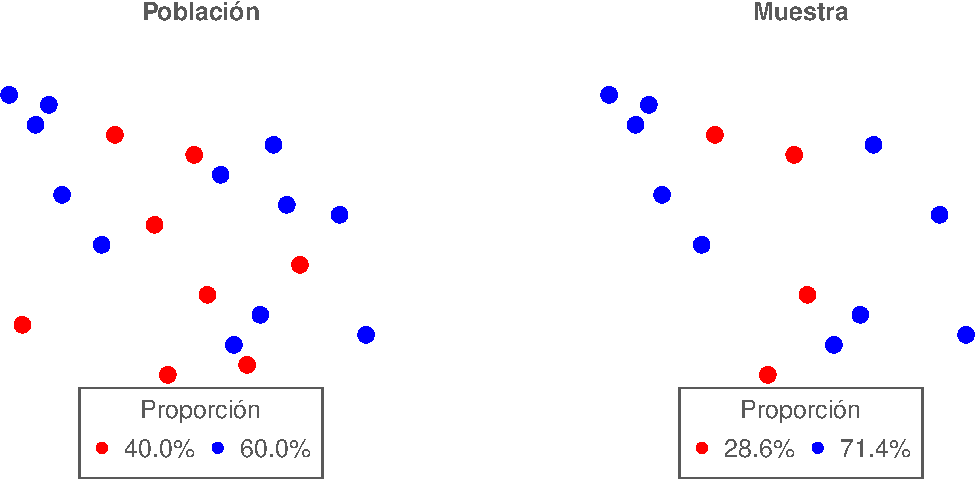
\includegraphics{est1+descriptiva_files/figure-latex/unnamed-chunk-2-1} \end{center}

\hypertarget{estimador-y-estimaciuxf3n}{%
\subsection*{Estimador y Estimación}\label{estimador-y-estimaciuxf3n}}
\addcontentsline{toc}{subsection}{Estimador y Estimación}

\begin{itemize}
\tightlist
\item
  \textbf{Estimador}: Un estimador es un estadístico usado para aproximar (incertidumbre) el valor de un parámetro. Usualmente no cambia la técnica entre la población y la muestra, por ejemplo, si deseo aproximar la proporción de bolitas rojas en la población, se usaría la proporción de bolitas rojas en la muestra.
\item
  \textbf{Estimación}: Una estimación es el número que resulta de aplicar el estimador a una muestra particular. Esto difiera levemente de la definición anterior, ya que en términos estrictos, el estimador solo es la ``fórmula'', y la estimación es el valor resultante al aplicar la fórmula. Sin embargo, hoy en día es muy común encontrar textos en donde el estimador se considera tanto para la fórmula como para el valor obtenido.
\end{itemize}

\begin{center}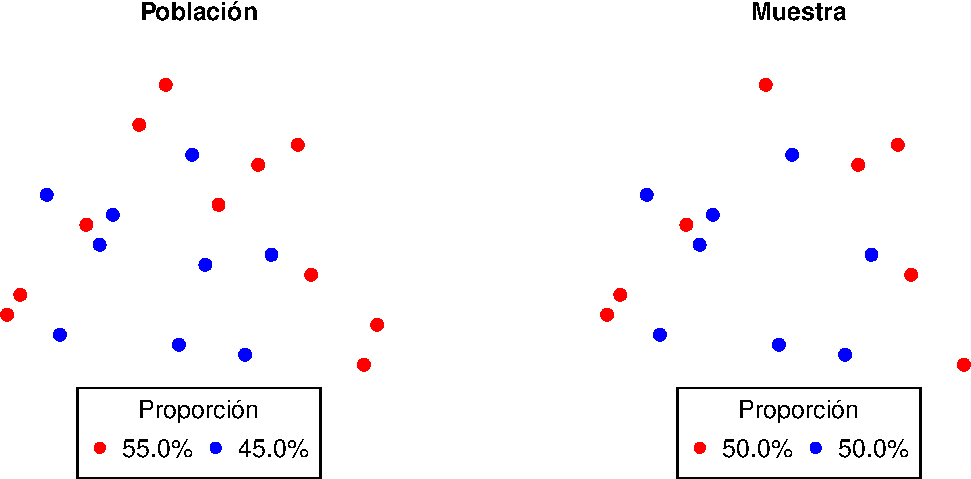
\includegraphics{est1+descriptiva_files/figure-latex/unnamed-chunk-3-1} \end{center}

¿Cuándo diríamos que una estimación es buena?

\hypertarget{variabilidad-muestral}{%
\subsection*{Variabilidad muestral}\label{variabilidad-muestral}}
\addcontentsline{toc}{subsection}{Variabilidad muestral}

Efectivamente, al estimación de un parámetro está fuertemente determinada por la muestra con la que uno trabaja. La forma en la que se elige una muestra es azarosa, por lo que es imposible saber de antemano si la estimación será buena o mala respecto al parámetro (error de estimación). En estadística, la forma en la que se elige o genera una muestra puede llegar a ser muy compleja, siendo un tema que está fuera del alcance de este curso. Cabe mencionar que en todo momento la elección es ``azarosa'\,', es decir, no podemos intencionarla en su totalidad.

El concepto detrás de esto es la variabilidad muestral, el cual, indica que dependiendo de la muestra que se obtenga de la población, esta se comportará distinto en relación al estadístico (igualmente para el valor del estimador: estimación).

\textbf{¿Cuál es la proporción de círculos rojos en la población relfejada en la figura \ref{fig:figura-poblacion1}?}

\begin{figure}

{\centering 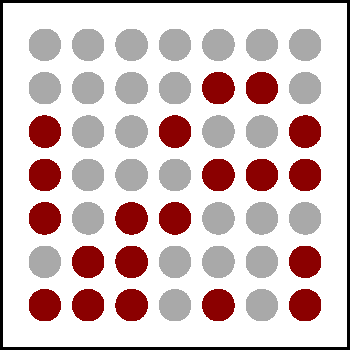
\includegraphics{est1+descriptiva_files/figure-latex/figura-poblacion1-1} 

}

\caption{Población}\label{fig:figura-poblacion1}
\end{figure}

\textbf{¿Qué podríamos inferir sobre el color predominante en la población en base a la muestra de la figura \ref{fig:figura-muestra1}?}

\begin{figure}

{\centering 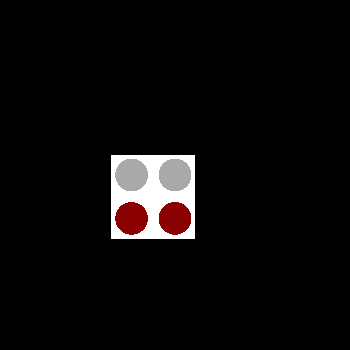
\includegraphics{est1+descriptiva_files/figure-latex/figura-muestra1-1} 

}

\caption{Muestra 1}\label{fig:figura-muestra1}
\end{figure}

\textbf{¿Y ahora? (Figura \ref{fig:figura-muestra2}) Diferentes muestras se comportan de manera diferente. Esto se denomina como variabilidad muestral}

\begin{figure}

{\centering 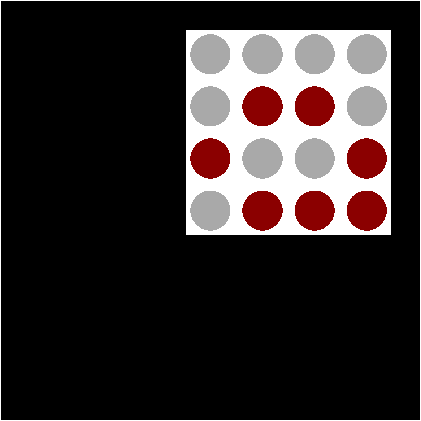
\includegraphics{est1+descriptiva_files/figure-latex/figura-muestra2-1} 

}

\caption{Muestra 2}\label{fig:figura-muestra2}
\end{figure}

\hypertarget{representatividad-y-sesgo-de-la-muestra}{%
\subsection*{Representatividad y sesgo de la muestra}\label{representatividad-y-sesgo-de-la-muestra}}
\addcontentsline{toc}{subsection}{Representatividad y sesgo de la muestra}

\textbf{Discusión}: Ambos conceptos se usan con frecuencia en la vida cotidiana, y a su vez están mal empleados. El sesgo no es una propiedad de la muestra sino que del estimador (concepto avanzado de estadística).

Por otro lado, la representatividad no es un concepto válido matemáticamente (no existe tal definición).

\hypertarget{medidas-de-tendencia-central-mtc}{%
\subsection*{Medidas de Tendencia Central (MTC)}\label{medidas-de-tendencia-central-mtc}}
\addcontentsline{toc}{subsection}{Medidas de Tendencia Central (MTC)}

\begin{itemize}
\tightlist
\item
  Media: \(\bar{x} = \displaystyle\frac{1}{n}\displaystyle\sum_{i=1}^n x_i\)
\item
  Mediana: La mediana de un conjunto de observaciones es el valor para el cual, cuando todas las observaciones se ordenan de manera creciente, la mitad de éstas es menor que este valor y la otra mitad.
\item
  Moda: La moda de un conjunto de observaciones es el valor de la observación que ocurre con mayor frecuencia en el conjunto.
\end{itemize}

\hypertarget{medidas-de-dipersiuxf3n-md}{%
\subsection*{Medidas de Dipersión (MD)}\label{medidas-de-dipersiuxf3n-md}}
\addcontentsline{toc}{subsection}{Medidas de Dipersión (MD)}

\begin{itemize}
\tightlist
\item
  Varianza: \(S^2 = \displaystyle{\frac{1}{n-1}\sum_{i=1}^n (x_i-\bar{x})^2}\)
\item
  Desviación Estándar: \(\sqrt{S}\)
\end{itemize}

\hypertarget{gruxe1ficos-descriptivos}{%
\section{Gráficos descriptivos}\label{gruxe1ficos-descriptivos}}

Los gráficos son una herramienta de resumen de información visual. Se usa tanto de forma descriptiva como analítica.

Para ilustrar los diferentes gráficos, usaremos la base de datos \emph{rock} que viene incluida en R, la cual, contiene mediciones de 48 muestras de roca de un yacimiento de petróleo. Los las columnas de esta base son:

\begin{itemize}
\tightlist
\item
  area: área del espacio de poros, en píxeles de 256 por 256.
\item
  peri: perímetro en píxeles.
\item
  shape: perímetros dividido por la raíz cuadrada del área.
\item
  perm: permeabilidad en mili-Darcies (unidad que se utiliza para cuantificar la capacidad de permeabilidad de un fluido a través de una roca; más información en este \href{https://en.wikipedia.org/wiki/Darcy_(unit)}{link}).
\end{itemize}

\hypertarget{histograma}{%
\subsection*{Histograma}\label{histograma}}
\addcontentsline{toc}{subsection}{Histograma}

Es la forma idónea para mostrar una tabla de frecuencia de forma visual. Se debe tener cuidado con la cantidad de intervalos del histograma, se recomienda utilizar la regla de Sturges (\(1+\log_2(n)\), aproximando hacia el entero más próximo).

\begin{Shaded}
\begin{Highlighting}[]
\FunctionTok{library}\NormalTok{(ggplot2)}
\NormalTok{datos }\OtherTok{=}\NormalTok{ rock}
\FunctionTok{ggplot}\NormalTok{(}\AttributeTok{data =}\NormalTok{ datos, }\FunctionTok{aes}\NormalTok{(}\AttributeTok{x =}\NormalTok{ perm)) }\SpecialCharTok{+}
  \FunctionTok{geom\_histogram}\NormalTok{(}\AttributeTok{color =} \StringTok{"white"}\NormalTok{, }\AttributeTok{fill =} \StringTok{"darkred"}\NormalTok{, }\AttributeTok{bins =} \DecValTok{7}\NormalTok{) }\SpecialCharTok{+}
  \FunctionTok{labs}\NormalTok{(}\AttributeTok{title =} \StringTok{"Histograma"}\NormalTok{, }\AttributeTok{x =} \StringTok{"Permeabilidad (mD)"}\NormalTok{, }\AttributeTok{y =} \StringTok{"Frecuencia"}\NormalTok{)}
\end{Highlighting}
\end{Shaded}

\begin{center}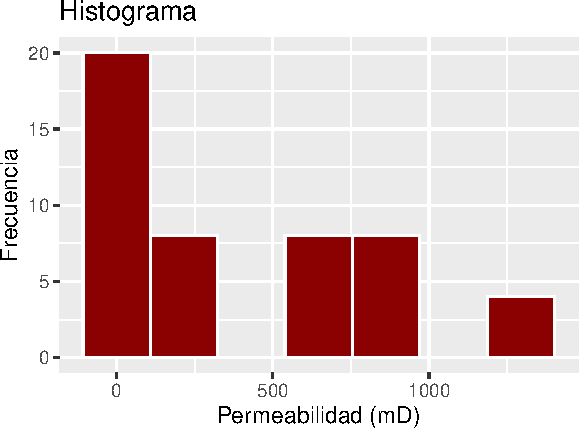
\includegraphics{est1+descriptiva_files/figure-latex/unnamed-chunk-4-1} \end{center}

\hypertarget{gruxe1fico-de-caja}{%
\subsection*{Gráfico de caja}\label{gruxe1fico-de-caja}}
\addcontentsline{toc}{subsection}{Gráfico de caja}

Este gráfico se utiliza para evidenciar las medidas de posición conocidas como cuartiles.

\begin{Shaded}
\begin{Highlighting}[]
\FunctionTok{ggplot}\NormalTok{(}\AttributeTok{data =}\NormalTok{ datos, }\FunctionTok{aes}\NormalTok{(}\AttributeTok{y =}\NormalTok{ perm)) }\SpecialCharTok{+} 
  \FunctionTok{geom\_boxplot}\NormalTok{(}\AttributeTok{color =} \StringTok{"black"}\NormalTok{, }\AttributeTok{fill =} \StringTok{"darkred"}\NormalTok{) }\SpecialCharTok{+}
  \FunctionTok{labs}\NormalTok{(}\AttributeTok{title =} \StringTok{"Caja"}\NormalTok{, }\AttributeTok{x =} \StringTok{"Permeabilidad (mD)"}\NormalTok{, }\AttributeTok{y =} \StringTok{"Dispersión/Cuantiles"}\NormalTok{) }
\end{Highlighting}
\end{Shaded}

\begin{center}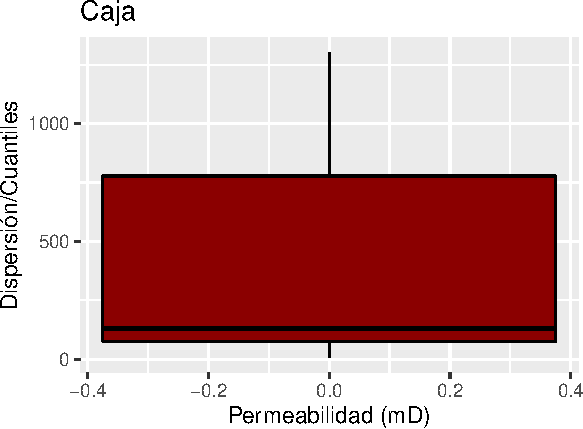
\includegraphics{est1+descriptiva_files/figure-latex/unnamed-chunk-5-1} \end{center}

\hypertarget{gruxe1fico-de-violuxedn}{%
\subsection*{Gráfico de violín}\label{gruxe1fico-de-violuxedn}}
\addcontentsline{toc}{subsection}{Gráfico de violín}

Gráfico utilizado para conocer la concentración de datos; es muy similar al histograma.

\begin{Shaded}
\begin{Highlighting}[]
\NormalTok{g }\OtherTok{=} \FunctionTok{ggplot}\NormalTok{(}\AttributeTok{data =}\NormalTok{ datos, }\FunctionTok{aes}\NormalTok{(}\AttributeTok{x =} \DecValTok{1}\NormalTok{, }\AttributeTok{y =}\NormalTok{ perm)) }\SpecialCharTok{+} 
  \FunctionTok{geom\_violin}\NormalTok{(}\AttributeTok{trim =}\NormalTok{ F, }\AttributeTok{alpha =} \FloatTok{0.5}\NormalTok{, }\AttributeTok{fill =} \StringTok{"aquamarine3"}\NormalTok{) }\SpecialCharTok{+}
  \FunctionTok{labs}\NormalTok{(}\AttributeTok{title =} \StringTok{"Violín"}\NormalTok{, }\AttributeTok{x =} \StringTok{""}\NormalTok{, }\AttributeTok{y =} \StringTok{"Permeabilidad (mD)"}\NormalTok{) }\SpecialCharTok{+} 
  \FunctionTok{theme}\NormalTok{(}\AttributeTok{axis.ticks.x =} \FunctionTok{element\_blank}\NormalTok{(),}
        \AttributeTok{axis.text.x =} \FunctionTok{element\_blank}\NormalTok{())}
\NormalTok{g}
\end{Highlighting}
\end{Shaded}

\begin{center}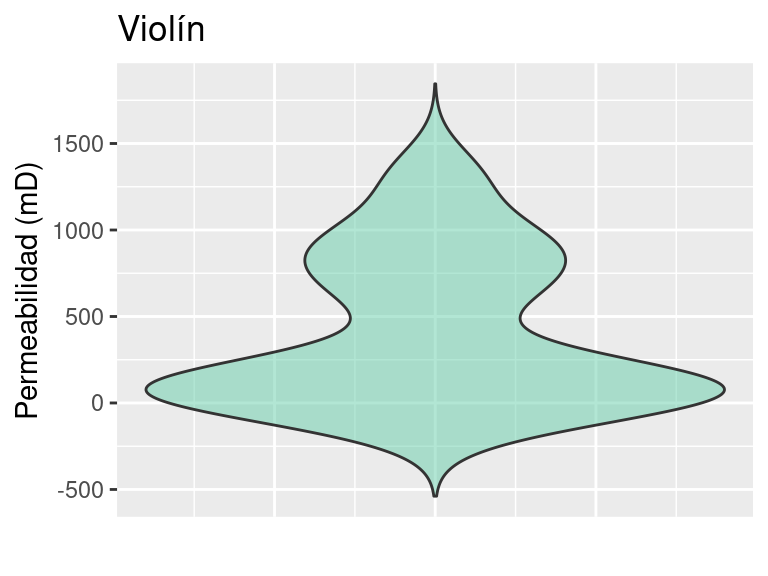
\includegraphics{est1+descriptiva_files/figure-latex/unnamed-chunk-6-1} \end{center}

\hypertarget{gruxe1fico-de-violuxedn-caja-promedio}{%
\subsection*{Gráfico de violín + caja + promedio}\label{gruxe1fico-de-violuxedn-caja-promedio}}
\addcontentsline{toc}{subsection}{Gráfico de violín + caja + promedio}

\begin{Shaded}
\begin{Highlighting}[]
\NormalTok{g }\SpecialCharTok{+} \FunctionTok{geom\_boxplot}\NormalTok{(}\AttributeTok{width =} \FloatTok{0.1}\NormalTok{, }\AttributeTok{color =} \StringTok{"black"}\NormalTok{,}
                 \AttributeTok{alpha =} \FloatTok{0.3}\NormalTok{, }\AttributeTok{fill =} \StringTok{"darkblue"}\NormalTok{)  }\SpecialCharTok{+}
  \FunctionTok{stat\_summary}\NormalTok{(}\AttributeTok{fun =}\NormalTok{ mean, }\AttributeTok{geom =} \StringTok{"point"}\NormalTok{,}
               \AttributeTok{size =} \DecValTok{1}\NormalTok{, }\AttributeTok{color =} \StringTok{"red"}\NormalTok{)}
\end{Highlighting}
\end{Shaded}

\begin{center}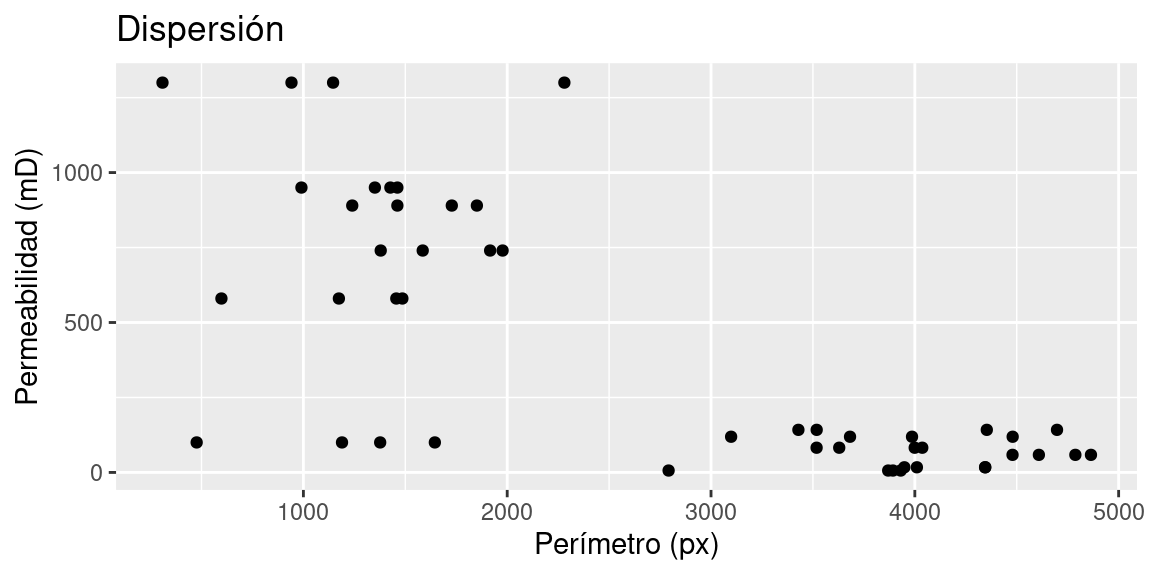
\includegraphics{est1+descriptiva_files/figure-latex/unnamed-chunk-7-1} \end{center}

\hypertarget{gruxe1fico-de-barras}{%
\subsection*{Gráfico de barras}\label{gruxe1fico-de-barras}}
\addcontentsline{toc}{subsection}{Gráfico de barras}

Gráfico por excelencia para visualizar la frecuencia de variables cualitativas.

\begin{Shaded}
\begin{Highlighting}[]
\NormalTok{datos}\SpecialCharTok{$}\NormalTok{Perm2 }\OtherTok{=} \FunctionTok{ifelse}\NormalTok{(datos}\SpecialCharTok{$}\NormalTok{perm }\SpecialCharTok{\textgreater{}} \DecValTok{500}\NormalTok{, }\StringTok{"Mayor a 500"}\NormalTok{, }\StringTok{"Menor a  500"}\NormalTok{)}
\FunctionTok{ggplot}\NormalTok{(}\AttributeTok{data =}\NormalTok{ datos,}\FunctionTok{aes}\NormalTok{(}\AttributeTok{x =}\NormalTok{ Perm2)) }\SpecialCharTok{+} 
  \FunctionTok{geom\_bar}\NormalTok{(}\AttributeTok{fill =} \StringTok{"darkgreen"}\NormalTok{) }\SpecialCharTok{+} 
  \FunctionTok{labs}\NormalTok{(}\AttributeTok{title =} \StringTok{"Barras"}\NormalTok{, }\AttributeTok{x =} \StringTok{"Permeabilidad (mD)"}\NormalTok{, }\AttributeTok{y =} \StringTok{"Frecuencia"}\NormalTok{)}
\end{Highlighting}
\end{Shaded}

\begin{center}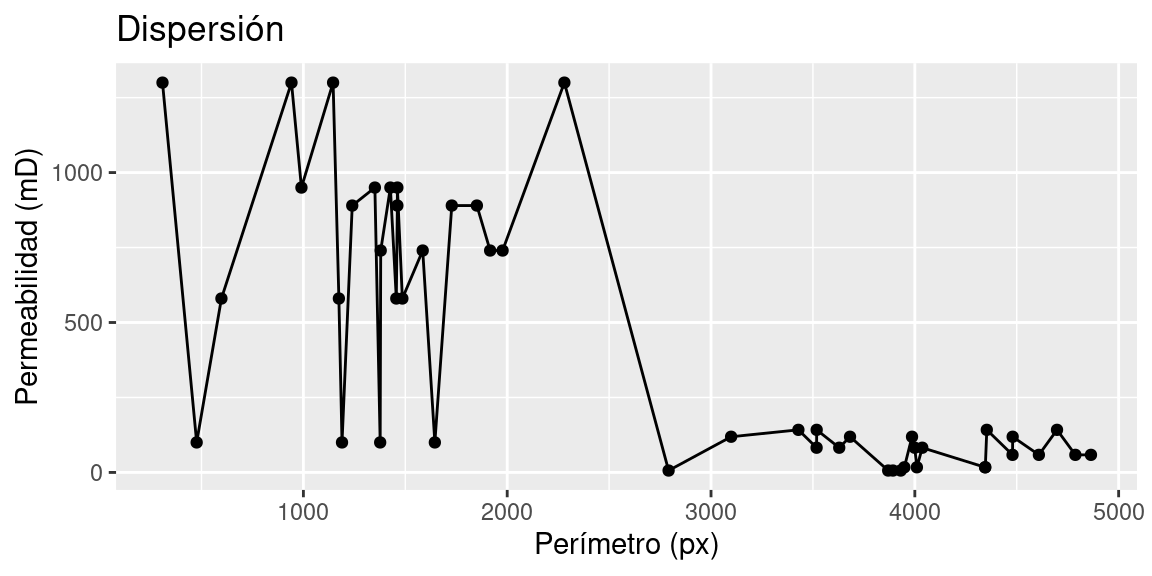
\includegraphics{est1+descriptiva_files/figure-latex/unnamed-chunk-8-1} \end{center}

\hypertarget{gruxe1fico-de-dispersiuxf3n}{%
\subsection*{Gráfico de dispersión}\label{gruxe1fico-de-dispersiuxf3n}}
\addcontentsline{toc}{subsection}{Gráfico de dispersión}

Gráfico que permite contrastar dos variables cuantitativas. En general, se usa para estudiar la asociación entre dos variables.

\begin{Shaded}
\begin{Highlighting}[]
\FunctionTok{ggplot}\NormalTok{(}\AttributeTok{data =}\NormalTok{ datos, }\FunctionTok{aes}\NormalTok{(}\AttributeTok{x =}\NormalTok{ peri, }\AttributeTok{y =}\NormalTok{ perm)) }\SpecialCharTok{+}
  \FunctionTok{geom\_point}\NormalTok{() }\SpecialCharTok{+}
  \FunctionTok{labs}\NormalTok{(}\AttributeTok{title =} \StringTok{"Dispersión"}\NormalTok{, }\AttributeTok{x =} \StringTok{"Perímetro (px)"}\NormalTok{, }\AttributeTok{y =} \StringTok{"Permeabilidad (mD)"}\NormalTok{)}
\end{Highlighting}
\end{Shaded}

\begin{center}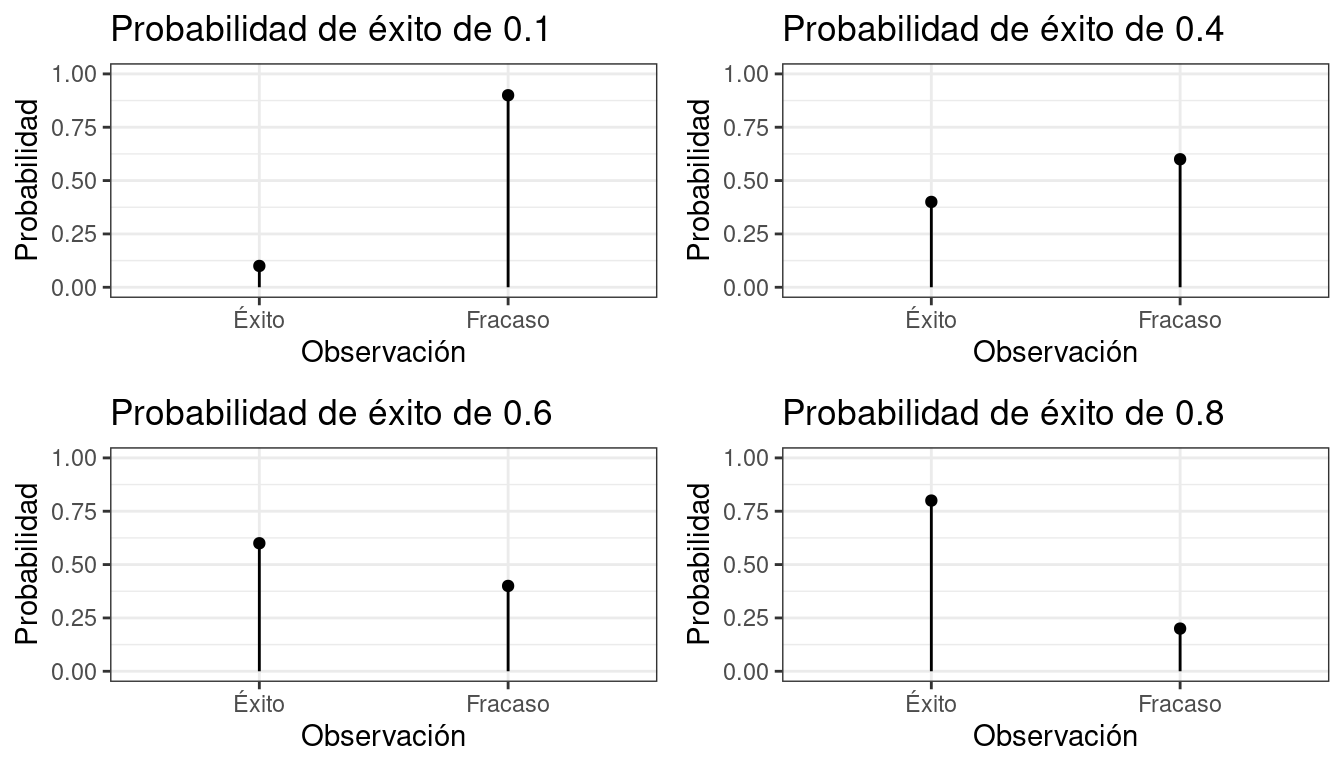
\includegraphics{est1+descriptiva_files/figure-latex/unnamed-chunk-9-1} \end{center}

\hypertarget{gruxe1fico-de-dispersiuxf3n-luxedneas}{%
\subsection*{Gráfico de dispersión + líneas}\label{gruxe1fico-de-dispersiuxf3n-luxedneas}}
\addcontentsline{toc}{subsection}{Gráfico de dispersión + líneas}

\begin{Shaded}
\begin{Highlighting}[]
\FunctionTok{ggplot}\NormalTok{(}\AttributeTok{data =}\NormalTok{ datos, }\FunctionTok{aes}\NormalTok{(}\AttributeTok{x =}\NormalTok{ peri, }\AttributeTok{y =}\NormalTok{ perm)) }\SpecialCharTok{+} 
  \FunctionTok{geom\_point}\NormalTok{() }\SpecialCharTok{+} 
  \FunctionTok{geom\_line}\NormalTok{() }\SpecialCharTok{+}
  \FunctionTok{labs}\NormalTok{(}\AttributeTok{title =} \StringTok{"Dispersión"}\NormalTok{, }\AttributeTok{x =} \StringTok{"Perímetro (px)"}\NormalTok{, }\AttributeTok{y =} \StringTok{"Permeabilidad (mD)"}\NormalTok{)}
\end{Highlighting}
\end{Shaded}

\begin{center}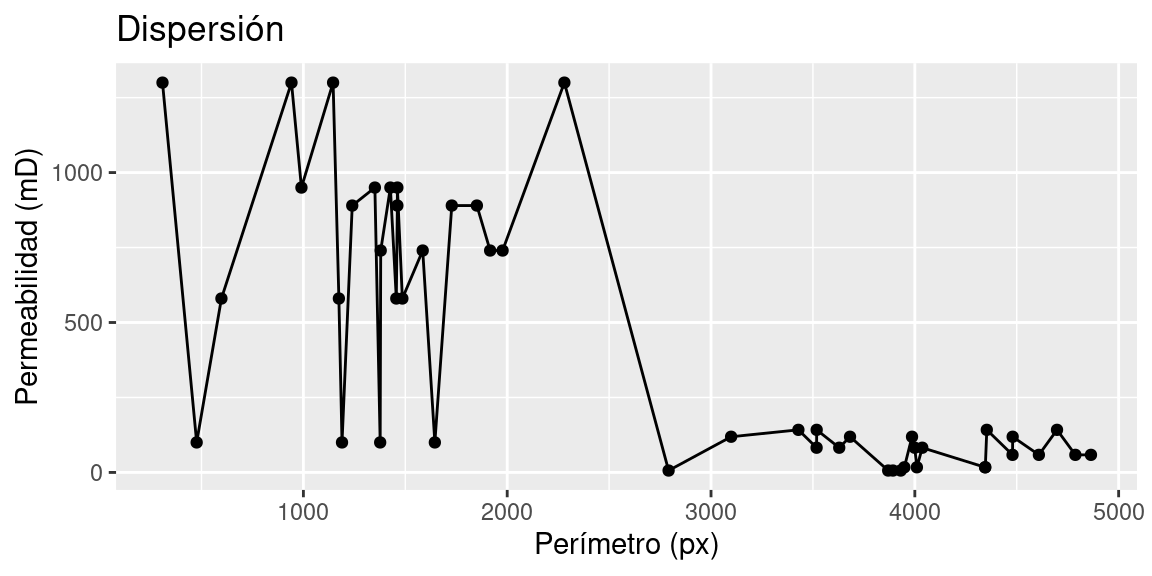
\includegraphics{est1+descriptiva_files/figure-latex/unnamed-chunk-10-1} \end{center}

\hypertarget{ejercicios}{%
\section{Ejercicios}\label{ejercicios}}

Desarrollar el \href{https://colab.research.google.com/drive/1wASaDklH5qgHqfCPdri-V2cg00KflJBf?usp=sharing}{Taller 1}.

\hypertarget{parts}{%
\chapter{Parts}\label{parts}}

You can add parts to organize one or more book chapters together. Parts can be inserted at the top of an .Rmd file, before the first-level chapter heading in that same file.

Add a numbered part: \texttt{\#\ (PART)\ Act\ one\ \{-\}} (followed by \texttt{\#\ A\ chapter})

Add an unnumbered part: \texttt{\#\ (PART\textbackslash{}*)\ Act\ one\ \{-\}} (followed by \texttt{\#\ A\ chapter})

Add an appendix as a special kind of un-numbered part: \texttt{\#\ (APPENDIX)\ Other\ stuff\ \{-\}} (followed by \texttt{\#\ A\ chapter}). Chapters in an appendix are prepended with letters instead of numbers.

\hypertarget{footnotes-and-citations}{%
\chapter{Footnotes and citations}\label{footnotes-and-citations}}

\hypertarget{footnotes}{%
\section{Footnotes}\label{footnotes}}

Footnotes are put inside the square brackets after a caret \texttt{\^{}{[}{]}}. Like this one \footnote{This is a footnote.}.

\hypertarget{citations}{%
\section{Citations}\label{citations}}

Reference items in your bibliography file(s) using \texttt{@key}.

For example, we are using the \textbf{bookdown} package \citep{R-bookdown} (check out the last code chunk in index.Rmd to see how this citation key was added) in this sample book, which was built on top of R Markdown and \textbf{knitr} \citep{xie2015} (this citation was added manually in an external file book.bib).
Note that the \texttt{.bib} files need to be listed in the index.Rmd with the YAML \texttt{bibliography} key.

The RStudio Visual Markdown Editor can also make it easier to insert citations: \url{https://rstudio.github.io/visual-markdown-editing/\#/citations}

\hypertarget{blocks}{%
\chapter{Blocks}\label{blocks}}

\hypertarget{equations}{%
\section{Equations}\label{equations}}

Here is an equation.

\begin{equation} 
  f\left(k\right) = \binom{n}{k} p^k\left(1-p\right)^{n-k}
  \label{eq:binom}
\end{equation}

You may refer to using \texttt{\textbackslash{}@ref(eq:binom)}, like see Equation \eqref{eq:binom}.

\hypertarget{theorems-and-proofs}{%
\section{Theorems and proofs}\label{theorems-and-proofs}}

Labeled theorems can be referenced in text using \texttt{\textbackslash{}@ref(thm:tri)}, for example, check out this smart theorem \ref{thm:tri}.

\begin{theorem}
\protect\hypertarget{thm:tri}{}\label{thm:tri}For a right triangle, if \(c\) denotes the \emph{length} of the hypotenuse
and \(a\) and \(b\) denote the lengths of the \textbf{other} two sides, we have
\[a^2 + b^2 = c^2\]
\end{theorem}

Read more here \url{https://bookdown.org/yihui/bookdown/markdown-extensions-by-bookdown.html}.

\hypertarget{callout-blocks}{%
\section{Callout blocks}\label{callout-blocks}}

The R Markdown Cookbook provides more help on how to use custom blocks to design your own callouts: \url{https://bookdown.org/yihui/rmarkdown-cookbook/custom-blocks.html}

\hypertarget{sharing-your-book}{%
\chapter{Sharing your book}\label{sharing-your-book}}

\hypertarget{publishing}{%
\section{Publishing}\label{publishing}}

HTML books can be published online, see: \url{https://bookdown.org/yihui/bookdown/publishing.html}

\hypertarget{pages}{%
\section{404 pages}\label{pages}}

By default, users will be directed to a 404 page if they try to access a webpage that cannot be found. If you'd like to customize your 404 page instead of using the default, you may add either a \texttt{\_404.Rmd} or \texttt{\_404.md} file to your project root and use code and/or Markdown syntax.

\hypertarget{metadata-for-sharing}{%
\section{Metadata for sharing}\label{metadata-for-sharing}}

Bookdown HTML books will provide HTML metadata for social sharing on platforms like Twitter, Facebook, and LinkedIn, using information you provide in the \texttt{index.Rmd} YAML. To setup, set the \texttt{url} for your book and the path to your \texttt{cover-image} file. Your book's \texttt{title} and \texttt{description} are also used.

This \texttt{gitbook} uses the same social sharing data across all chapters in your book- all links shared will look the same.

Specify your book's source repository on GitHub using the \texttt{edit} key under the configuration options in the \texttt{\_output.yml} file, which allows users to suggest an edit by linking to a chapter's source file.

Read more about the features of this output format here:

\url{https://pkgs.rstudio.com/bookdown/reference/gitbook.html}

Or use:

\begin{Shaded}
\begin{Highlighting}[]
\NormalTok{?bookdown}\SpecialCharTok{::}\NormalTok{gitbook}
\end{Highlighting}
\end{Shaded}


  \bibliography{book.bib,packages.bib}

\end{document}
